% This file was created with tikzplotlib v0.10.1.
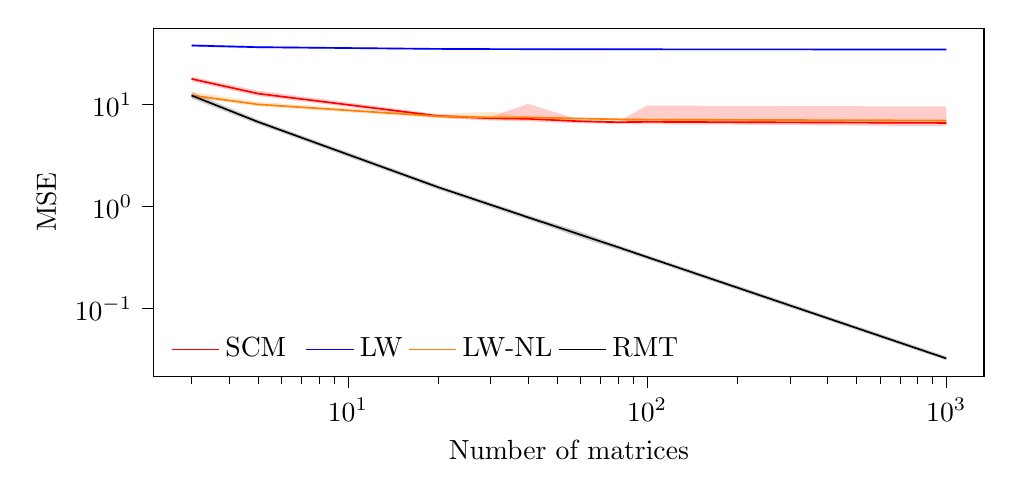
\begin{tikzpicture}

\definecolor{crimson2143940}{RGB}{214,39,40}
\definecolor{darkgray176}{RGB}{176,176,176}
\definecolor{darkorange25512714}{RGB}{255,127,14}
\definecolor{forestgreen4416044}{RGB}{44,160,44}
\definecolor{lightgray204}{RGB}{204,204,204}
\definecolor{steelblue31119180}{RGB}{31,119,180}

\begin{axis}[
width=\columnwidth,
height=6cm,
legend cell align={left},
legend columns=4, 
legend style={draw=none, at={(0.01, 0.01)},anchor=south west, /tikz/column 2/.style={column sep=5pt,}},
log basis x={10},
log basis y={10},
tick align=outside,
tick pos=left,
x grid style={darkgray176},
xlabel={Number of matrices},
xmin=2.2437647322819, xmax=1337.03857487278,
xmode=log,
xtick style={color=black},
minor xtick={2,3,4,5,6,7,8,9,20,30,40,50,60,70,80,90,200,300,400,500,600,700,800,900,2000,3000,4000,5000,6000,7000,8000,9000},
xtick={0.1,1,10,100,1000,10000,100000},
xticklabels={
  \(\displaystyle {10^{-1}}\),
  \(\displaystyle {10^{0}}\),
  \(\displaystyle {10^{1}}\),
  \(\displaystyle {10^{2}}\),
  \(\displaystyle {10^{3}}\),
  \(\displaystyle {10^{4}}\),
  \(\displaystyle {10^{5}}\)
},
y grid style={darkgray176},
ylabel={MSE},
ymin=0.0218043651445638, ymax=56.0024815737763,
ymode=log,
ytick style={color=black},
ytick={0.001,0.01,0.1,1,10,100,1000},
yticklabels={
  \(\displaystyle {10^{-3}}\),
  \(\displaystyle {10^{-2}}\),
  \(\displaystyle {10^{-1}}\),
  \(\displaystyle {10^{0}}\),
  \(\displaystyle {10^{1}}\),
  \(\displaystyle {10^{2}}\),
  \(\displaystyle {10^{3}}\)
}
]
\path [fill=red, fill opacity=0.2]
(axis cs:3,18.8043389613054)
--(axis cs:3,16.8314875609603)
--(axis cs:5,12.1381896526981)
--(axis cs:20,7.40333054447914)
--(axis cs:30,6.99241936580442)
--(axis cs:40,6.84333140532385)
--(axis cs:60,6.5547090007593)
--(axis cs:80,6.44242941841111)
--(axis cs:100,6.42923176293192)
--(axis cs:1000,6.15031714334588)
--(axis cs:1000,9.57269828056928)
--(axis cs:1000,9.57269828056928)
--(axis cs:100,9.77214297162595)
--(axis cs:80,6.84651314814767)
--(axis cs:60,7.03283275125054)
--(axis cs:40,10.1446648799031)
--(axis cs:30,7.5899688263652)
--(axis cs:20,8.04034681130094)
--(axis cs:5,13.6925881202131)
--(axis cs:3,18.8043389613054)
--cycle;

\path [fill=blue, fill opacity=0.2]
(axis cs:3,39.005998009636)
--(axis cs:3,36.8707156277165)
--(axis cs:5,35.5865352644737)
--(axis cs:20,34.5473070558395)
--(axis cs:30,34.579891613708)
--(axis cs:40,34.5237197996682)
--(axis cs:60,34.5172640777862)
--(axis cs:80,34.5040367785707)
--(axis cs:100,34.5406761244513)
--(axis cs:1000,34.6100474756888)
--(axis cs:1000,34.7667457265176)
--(axis cs:1000,34.7667457265176)
--(axis cs:100,35.018072659898)
--(axis cs:80,35.0204169989352)
--(axis cs:60,35.1346156589806)
--(axis cs:40,35.3105106802022)
--(axis cs:30,35.4543696924228)
--(axis cs:20,35.6181967536497)
--(axis cs:5,37.4501666134047)
--(axis cs:3,39.005998009636)
--cycle;

% \path [fill=forestgreen4416044, fill opacity=0.2]
% (axis cs:3,39.1942675122421)
% --(axis cs:3,37.2808363913984)
% --(axis cs:5,35.7911711661596)
% --(axis cs:20,34.8860863353065)
% --(axis cs:30,34.8716226124352)
% --(axis cs:40,34.7987963431535)
% --(axis cs:60,34.7593184055425)
% --(axis cs:80,34.7893520398673)
% --(axis cs:100,34.7844604342404)
% --(axis cs:1000,34.8937987135023)
% --(axis cs:1000,35.0518189132013)
% --(axis cs:1000,35.0518189132013)
% --(axis cs:100,35.2747395820992)
% --(axis cs:80,35.280664789503)
% --(axis cs:60,35.3843482742359)
% --(axis cs:40,35.491153530183)
% --(axis cs:30,35.7177289930558)
% --(axis cs:20,35.9151745882271)
% --(axis cs:5,37.7412903329415)
% --(axis cs:3,39.1942675122421)
% --cycle;

\path [fill=orange, fill opacity=0.2]
(axis cs:3,13.4150106353578)
--(axis cs:3,11.6981243465868)
--(axis cs:5,9.61827227403283)
--(axis cs:20,7.36444461877267)
--(axis cs:30,7.14352133961181)
--(axis cs:40,7.00841372147705)
--(axis cs:60,6.94320751913582)
--(axis cs:80,6.91012783163816)
--(axis cs:100,6.74522525628883)
--(axis cs:1000,6.69264725683738)
--(axis cs:1000,6.94221203330159)
--(axis cs:1000,6.94221203330159)
--(axis cs:100,7.30551547212458)
--(axis cs:80,7.36045805216695)
--(axis cs:60,7.29151580346628)
--(axis cs:40,7.60690213210427)
--(axis cs:30,8.48945039975636)
--(axis cs:20,8.00543821354113)
--(axis cs:5,10.6273361853284)
--(axis cs:3,13.4150106353578)
--cycle;

\path [fill=black, fill opacity=0.2]
(axis cs:3,13.2493448302234)
--(axis cs:3,11.4860534270566)
--(axis cs:5,6.42575481512846)
--(axis cs:20,1.47633412090066)
--(axis cs:30,0.984704248724723)
--(axis cs:40,0.745685316007821)
--(axis cs:60,0.495193991616838)
--(axis cs:80,0.37902380712767)
--(axis cs:100,0.304820634372988)
--(axis cs:1000,0.0311550294148225)
--(axis cs:1000,0.0341197901365598)
--(axis cs:1000,0.0341197901365598)
--(axis cs:100,0.335310339716903)
--(axis cs:80,0.418883868889403)
--(axis cs:60,0.564439336906844)
--(axis cs:40,0.825173648165352)
--(axis cs:30,1.09302438447952)
--(axis cs:20,1.6280331731264)
--(axis cs:5,7.12816348512381)
--(axis cs:3,13.2493448302234)
--cycle;

\addplot [semithick, red]
table {%
3 17.8578669661773
5 12.8155686738752
20 7.73639624547268
30 7.34216999141405
40 7.25532560940202
60 6.85056244981613
80 6.72031984059409
100 6.7701088293971
1000 6.60524420674127
};
\addlegendentry{SCM}
\addplot [semithick, blue]
table {%
3 37.9287812137695
5 36.510870869585
20 35.1182093437605
30 34.9814035545661
40 34.8926849163795
60 34.8302189752921
80 34.7929360698527
100 34.7916496247899
1000 34.6521177061983
};
\addlegendentry{LW}
% \addplot [semithick, forestgreen4416044]
% table {%
% 3 38.1727186345762
% 5 36.786643404877
% 20 35.3985798037799
% 30 35.2478541588808
% 40 35.1524144312998
% 60 35.0782768971115
% 80 35.0594873887069
% 100 35.0314417745551
% 1000 34.9673991259342
% };
% \addlegendentry{OAS}
\addplot [semithick, orange]
table {%
3 12.3112936200546
5 10.0392129332778
20 7.68102260267098
30 7.48727072899839
40 7.50180091565585
60 7.30395299485244
80 7.16727107641064
100 7.12028507303887
1000 6.98447855227814
};
\addlegendentry{LW-NL}
\addplot [semithick, black]
table {%
3 12.279626119493
5 6.77618065458479
20 1.55136016011359
30 1.04161989750938
40 0.785323043157254
60 0.528655778789545
80 0.399959956704565
100 0.320227137484716
1000 0.0325302658364751
};
\addlegendentry{RMT}

\end{axis}

\end{tikzpicture}
